\subsection{Sky-Timelapse: Causal Results}\label{sec:causal_sky_timelapse}

We use the same frame counts and discretization step counts as in the other experiments. Here, we do causal (regular autoregressive) generation, where we don't prompt with the future, but rather, only give a prefix of 1 or 4 frames.

See Tables \ref{tab:sky_causal_rollout_fvd} (FVD), \ref{tab:sky_causal_rollout_fid} (FID), Figure \ref{tab:pareto_sky_timelapse_causal} (combined ranking).
Under this setting, \textit{ABC without Brownian Bridge is Pareto-optimal} (Figure \ref{tab:pareto_sky_timelapse_causal}) across FVD and FID scores on causal rollout. As compared to the conditional diffusion bridge methods on the Pareto front, we see that ABC has low discrepancy in its overall FID (3) and FVD (2) rankings, indicating consistency and robustness across multiple aspects of quality measure.


%Table \ref{tab:sky_causal_overall_avg_rank} is an aggregation of the overall ranking in causal FID and the overall ranking in causal FVD (similar to Tables \ref{tab:sky_non_causal_overall_avg_rank}, \ref{tab:celebvhq_non_causal_overall_avg_rank}).

% We see that while under this causal setting, ABC no longer ranks first, ABC without Brownian Bridge is still competitive with the best conditional diffusion bridge baselines. Furthermore, digging deeper into the metrics, we see that the $\sigma=0.3$ conditional bridge baseline (1st place) that beat ABC w/o BB (2nd place) on FVD score usually \textit{ranked below ABC w/o BB on FID}.

% This can also be gleaned from the standard deviations (since this was calculated from two samples, it is half the difference between FID and FVD rankings) in Table \ref{tab:sky_causal_overall_avg_rank}. They show that ABC w/o BB, although it comes in second by average rank, has a much lower variation in its FID vs FVD ranks ($2.50 \pm 0.38$), as opposed to the first-place $\sigma=0.3$ conditional diffusion bridge's widely varying rank ($2.31 \pm 1.31$). This implies that \textit{ABC w/o BB is more consistent and robust across metrics}.

\begin{table}[h]
\centering\tiny
\caption{Sky-timelapse --- Causal --- FVD ($\downarrow$)}
\label{tab:sky_causal_rollout_fvd}
\begin{tabular}{lrrrrrrrr}
\toprule
 & \multicolumn{4}{c}{Num Frames = 32} & \multicolumn{4}{c}{Num Frames = 16} \\
\cmidrule(lr){2-5} \cmidrule(lr){6-9}
 & \multicolumn{2}{c}{prefix\_length = 1} & \multicolumn{2}{c}{prefix\_length = 4} & \multicolumn{2}{c}{prefix\_length = 1} & \multicolumn{2}{c}{prefix\_length = 4} \\
\cmidrule(lr){2-3} \cmidrule(lr){4-5} \cmidrule(lr){6-7} \cmidrule(lr){8-9}
\textbf{Method} \ \ \ \ \ \ Steps & \multicolumn{1}{c}{250} & \multicolumn{1}{c}{500} & \multicolumn{1}{c}{250} & \multicolumn{1}{c}{500} & \multicolumn{1}{c}{250} & \multicolumn{1}{c}{500} & \multicolumn{1}{c}{250} & \multicolumn{1}{c}{500} \\
\midrule
\rowcolor{gray!20} \multicolumn{9}{l}{\textit{ABC}} \\
\quad No BB: $\sigma$=0.4 & \textbf{\textit{374.0}} & \textbf{\textit{284.6}} & \textbf{\textit{359.4}} & \textbf{\textit{277.5}} & \textbf{\textit{247.3}} & \textbf{\textit{208.3}} & \textbf{\textit{188.5}} & 164.1 \\
\quad W/ BB: $\sigma$=0.4 & 461.3 & 367.4 & 416.6 & 326.7 & 306.0 & 240.4 & 224.6 & 182.1 \\
\rowcolor{gray!20} \multicolumn{9}{l}{\textit{Conditional Diffusion Bridge}} \\
\quad $\sigma=0.071$ & 487.1 & 427.0 & 438.9 & 359.9 & 398.6 & 352.7 & 308.6 & 281.9 \\
\quad $\sigma=0.1$ & 411.6 & 329.5 & 388.9 & 314.8 & 327.6 & 275.4 & 249.1 & 222.8 \\
\quad $\sigma=0.3$ & \textbf{302.0} & \textbf{224.2} & \textbf{276.6} & \textbf{193.5} & \textbf{205.3} & \textbf{184.2} & \textbf{157.2} & \textbf{137.4} \\
\quad $\sigma=0.4$ & 440.9 & 311.0 & 434.6 & 290.0 & 269.6 & 214.5 & 219.7 & \textbf{\textit{160.0}} \\
\quad $\sigma=0.6$ & 742.2 & 552.9 & 750.4 & 562.6 & 458.1 & 299.7 & 433.5 & 279.0 \\
\rowcolor{gray!20} \multicolumn{9}{l}{\textit{Noise-to-Data Diffusion}} \\
\quad Cos: (3.0, 0.04) & 700.3 & 511.1 & 748.2 & 504.3 & 504.6 & 258.5 & 476.7 & 213.7 \\
\quad Cos: (5.0, 0.05) & 861.8 & 783.4 & 927.2 & 844.8 & 762.6 & 361.6 & 752.8 & 322.9 \\
\quad Exp: (4.0, 2.5) & 765.3 & 658.7 & 617.7 & 534.3 & 618.8 & 320.9 & 417.3 & 211.5 \\
\quad Exp: (5.0, 5.0) & 797.0 & 680.2 & 643.6 & 579.0 & 694.5 & 411.6 & 469.7 & 304.1 \\
\bottomrule
\end{tabular}
\end{table}

\begin{table}[h]
\centering\tiny
\caption{Sky-timelapse --- Causal --- FID ($\downarrow$)}
\label{tab:sky_causal_rollout_fid}
\begin{tabular}{lrrrrrrrr}
\toprule
 & \multicolumn{4}{c}{Num Frames = 32} & \multicolumn{4}{c}{Num Frames = 16} \\
\cmidrule(lr){2-5} \cmidrule(lr){6-9}
 & \multicolumn{2}{c}{prefix\_length = 1} & \multicolumn{2}{c}{prefix\_length = 4} & \multicolumn{2}{c}{prefix\_length = 1} & \multicolumn{2}{c}{prefix\_length = 4} \\
\cmidrule(lr){2-3} \cmidrule(lr){4-5} \cmidrule(lr){6-7} \cmidrule(lr){8-9}
\textbf{Method} \ \ \ \ \ \ Steps & \multicolumn{1}{c}{250} & \multicolumn{1}{c}{500} & \multicolumn{1}{c}{250} & \multicolumn{1}{c}{500} & \multicolumn{1}{c}{250} & \multicolumn{1}{c}{500} & \multicolumn{1}{c}{250} & \multicolumn{1}{c}{500} \\
\midrule
\rowcolor{gray!20} \multicolumn{9}{l}{\textit{ABC}} \\
\quad No BB: $\sigma$=0.4 & 20.1 & 14.0 & 17.2 & 12.2 & 10.3 & 8.6 & \textbf{6.6} & 5.5 \\
\quad W/ BB: $\sigma$=0.4 & 25.1 & 17.2 & 21.5 & 14.9 & 12.6 & 10.5 & 8.0 & 6.6 \\
\rowcolor{gray!20} \multicolumn{9}{l}{\textit{Conditional Diffusion Bridge}} \\
\quad $\sigma=0.071$ & \textbf{14.0} & \textbf{9.9} & \textbf{15.2} & \textbf{10.8} & \textbf{8.6} & \textbf{6.6} & 8.0 & 5.9 \\
\quad $\sigma=0.1$ & \textbf{\textit{17.9}} & \textbf{\textit{13.0}} & \textbf{\textit{15.6}} & \textbf{\textit{11.3}} & \textbf{\textit{9.4}} & \textbf{\textit{7.5}} & 6.7 & \textbf{\textit{5.2}} \\
\quad $\sigma=0.3$ & 43.7 & 19.8 & 29.9 & 14.2 & 11.8 & 7.9 & \textbf{\textit{6.6}} & \textbf{4.7} \\
\quad $\sigma=0.4$ & 96.2 & 38.4 & 68.3 & 27.2 & 20.2 & 10.9 & 11.3 & 6.3 \\
\quad $\sigma=0.6$ & 220.4 & 121.8 & 171.2 & 95.0 & 59.5 & 25.3 & 35.0 & 15.3 \\
\rowcolor{gray!20} \multicolumn{9}{l}{\textit{Noise-to-Data Diffusion}} \\
\quad Cos: (3.0, 0.04) & 175.1 & 38.9 & 140.4 & 28.0 & 29.2 & 12.1 & 16.2 & 6.6 \\
\quad Cos: (5.0, 0.05) & 245.9 & 87.9 & 203.0 & 68.4 & 63.0 & 17.6 & 37.7 & 9.9 \\
\quad Exp: (4.0, 2.5) & 192.1 & 141.7 & 159.9 & 116.1 & 84.0 & 18.7 & 49.9 & 9.8 \\
\quad Exp: (5.0, 5.0) & 211.6 & 145.7 & 181.4 & 117.9 & 90.8 & 26.7 & 55.5 & 14.3 \\
\bottomrule
\end{tabular}
\end{table}

\begin{figure}[h]
    \centering
    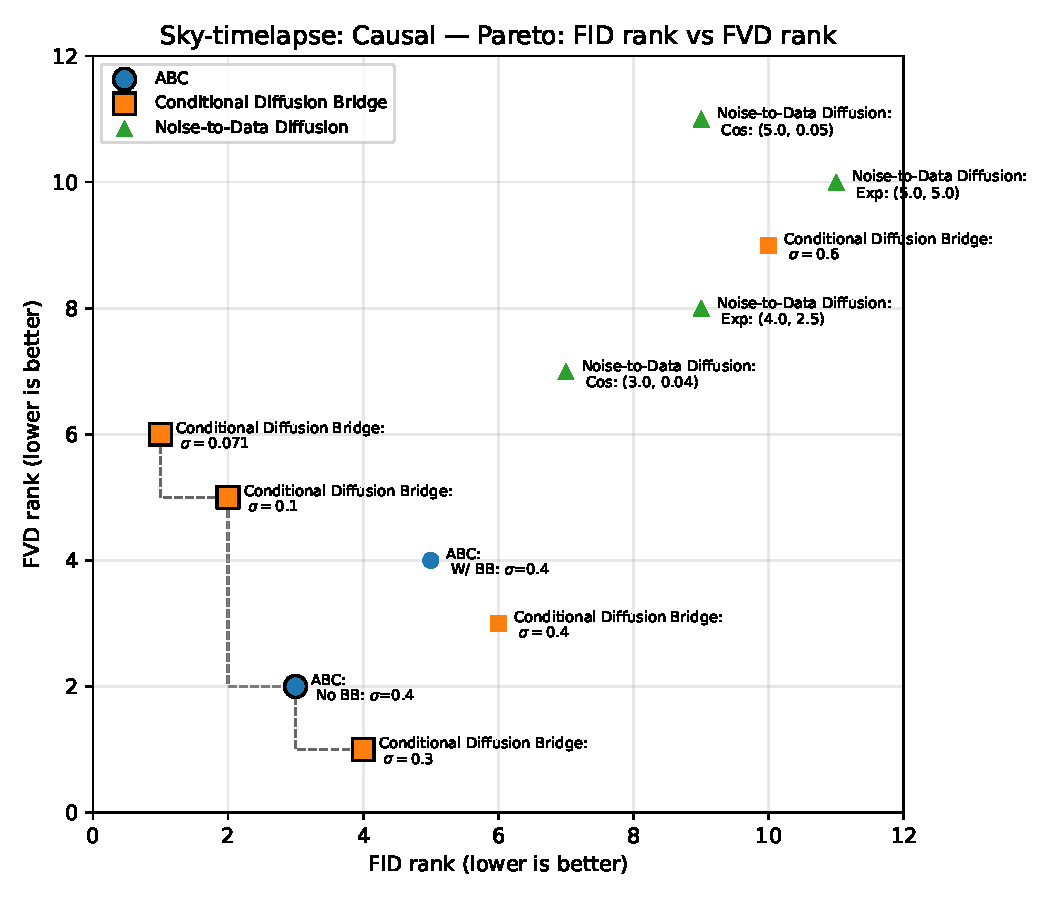
\includegraphics[width=0.7\linewidth]{results_numbers_and_figures/sky_timelapse_pareto_causal_rollout.pdf}
    \caption{\textbf{Pareto Front for Sky-Timelapse Causal Generation:} ABC is Pareto-optimal across FVD and FID scores for causally-ordered generation on Sky-Timelapse. Corresponds to results in Tables \ref{tab:sky_causal_rollout_fid}, \ref{tab:sky_causal_rollout_fvd}. Horizontal axis is the ordering of average rank in Table \ref{tab:sky_causal_rollout_fid}'s columns, and vertical axis is the ordering of average rank in Table \ref{tab:sky_causal_rollout_fvd}'s columns.}\label{tab:pareto_sky_timelapse_causal}
\end{figure}

% % Put this in the appendix
% \begin{table}[htbp]
% \centering
% \caption{Sky-timelapse (Causal) --- Average Rank Across Metrics  ($\downarrow$). Average rank from Tables \ref{tab:sky_causal_rollout_fid}, \ref{tab:sky_causal_rollout_fvd}.}
% \label{tab:sky_causal_overall_avg_rank}
% \begin{tabular}{lcc}
% \toprule
% Method & Avg Rank & Overall Rank \\
% \midrule
% \rowcolor{gray!20} \multicolumn{3}{l}{\textit{ABC}} \\
% \quad No BB: $\sigma$=0.4 & \textbf{\textit{2.50}} $\pm$ 0.38 & 2 \\
% \quad W/ BB: $\sigma$=0.4 & 4.56 $\pm$ 0.19 & 5 \\
% \rowcolor{gray!20} \multicolumn{3}{l}{\textit{Conditional Diffusion Bridge}} \\
% \quad $\sigma=0.071$ & 4.31 $\pm$ 2.44 & 4 \\
% \quad $\sigma=0.1$ & 3.38 $\pm$ 1.25 & 3 \\
% \quad $\sigma=0.3$ & \textbf{2.31} $\pm$ 1.31 & 1 \\
% \quad $\sigma=0.4$ & 4.56 $\pm$ 1.31 & 6 \\
% \quad $\sigma=0.6$ & 8.69 $\pm$ 0.56 & 9 \\
% \rowcolor{gray!20} \multicolumn{3}{l}{\textit{Noise-to-Data Diffusion}} \\
% \quad Cos: (3.0, 0.04) & 7.12 $\pm$ 0.25 & 7 \\
% \quad Cos: (5.0, 0.05) & 10.00 $\pm$ 0.88 & 10 \\
% \quad Exp: (4.0, 2.5) & 8.44 $\pm$ 0.69 & 8 \\
% \quad Exp: (5.0, 5.0) & 10.12 $\pm$ 0.38 & 11 \\
% \bottomrule
% \end{tabular}
% \end{table}
